\documentclass[11pt]{article}

\usepackage{amsmath,amsfonts,amssymb,graphicx,setspace,authblk}
\usepackage{titlesec,blkarray, bm} 
\usepackage{float,afterpage}
\usepackage[running,mathlines]{lineno}
\usepackage[vmargin=1in,hmargin=1in]{geometry}
\usepackage[authoryear,sort]{natbib}
\usepackage[dvipsnames]{xcolor}
\usepackage{hyperref}

\usepackage{enumitem}
\setlist{topsep=.125em,itemsep=-0.15em,leftmargin=0.75cm}
\setlength{\parindent}{0.35in}

\usepackage[sc]{mathpazo} %Like Palatino with extensive math support

% Coloring of R code listings
\usepackage[formats]{listings}
\usepackage{color}
\definecolor{mygreen}{rgb}{0.1,0.5,0.1}
\definecolor{mygray}{rgb}{0.5,0.5,0.5}
\definecolor{mymauve}{rgb}{0.58,0,0.82}
\definecolor{mygrey}{rgb}{0.3,0.3,0.1}
\lstset{
language=R,
otherkeywords={data.frame},
basicstyle=\normalsize\ttfamily, 
commentstyle=\normalsize\ttfamily,
keywordstyle=\normalsize\ttfamily,
stringstyle=\color{mymauve}, 
commentstyle=\color{mygreen},
keywordstyle=\color{blue},
showstringspaces=false, xleftmargin=2.5ex,
columns=flexible,
literate={~}{{$\sim \; \; $}}1,
alsodigit={\.,\_},
deletekeywords={on,by,data,R,Q,mean,var,sd,log,family,na,options,q,weights,effects,matrix,nrow,ncol,wt,fix,distance},
}
\lstset{escapeinside={(*}{*)}} 

\lstdefineformat{Rpretty}{
	; = \space,
	\, = [\ \,\]]\string\space,
	<- = [\ ]\space\string\space,
	\= = [\ ]\space\string\space}


\usepackage{lineno}
\renewcommand{\refname}{Literature Cited}
\renewcommand{\floatpagefraction}{0.98}
\renewcommand{\topfraction}{0.99}
\renewcommand{\textfraction}{0.05}

\clubpenalty = 10000
\widowpenalty = 10000

\sloppy 

\usepackage{ifpdf}
\ifpdf
\DeclareGraphicsExtensions{.pdf,.png,.jpg}
\usepackage{epstopdf}
\else
\DeclareGraphicsExtensions{.eps}
\fi

\DeclareMathOperator{\Ex}{\mathbb{E}}
\DeclareMathOperator{\var}{\textit{Var}}
\DeclareMathOperator{\cov}{\textit{Cov}}



%%%%%%%%% Macros to simplify using our notation 

\newcommand{\s}[1]{{#1}^{\#}}
\newcommand{\f}[1]{{#1}^{\flat}}
\newcommand{\sr}[1]{{#1}^{*}}
\newcommand{\br}[1]{\langle {#1} \rangle} 
\newcommand{\bs}{\backslash} 
\def\alphat{\widetilde{\alpha}}
\newcommand{\half}{\frac{1}{2}}

% commands for commenting
\newcommand{\tom}[2]{{\color{red}{#1}}\footnote{\textit{\color{red}{#2}}}}
\newcommand{\steve}[2]{{\color{blue}{#1}}\footnote{\textit{\color{blue}{#2}}}}

% Define Box environment for numbered boxes. 
\newcounter{box}
\newcommand{\boxnumber}{\addtocounter{box}{1} \thebox \thinspace}

\floatstyle{boxed}
\newfloat{Box}{tbph}{box}

%%%%%%%%%%%%%%%%%%%%%%%%%%%%%%%%%%%%%%%%%%%%% 
%%% Just for commenting
%%%%%%%%%%%%%%%%%%%%%%%%%%%%%%%%%%%%%%%%%%%%
\usepackage[dvipsnames]{xcolor}
\newcommand{\comment}{\textcolor{blue}}
\newcommand{\new}{\textcolor{red}}

\newcommand{\be}{\begin{equation}}
\newcommand{\ee}{\end{equation}}

\newcommand{\red}{\textcolor{red}}

\title{My, how you've grown: a practical guide to modeling size transitions for Integral Projection Model (IPM) applications}

\author[a]{Tom E.X. Miller\thanks{Corresponding author. Department of BioSciences, Rice University,
Houston, TX 77005-1827. Email: tom.miller@rice.edu Phone: 713-348-4218}}
\author[b]{Stephen P. Ellner}
\affil[a]{Department of BioSciences, Rice University,Houston, TX } 
\affil[b]{Department of Ecology and Evolutionary Biology, Cornell University, Ithaca, New York} 

\renewcommand\Authands{ and }

\sloppy

\begin{document}

\renewcommand{\baselinestretch}{1.25} 
\maketitle

\bigskip 

\noindent \textbf{Authorship statement:} All authors discussed all aspects of the research and
contributed to developing methods, analyzing data, and writing and revising the paper.  

\bigskip 

\noindent{\textbf{Data accessibility statement}: No original data appear in this paper. 
Should the paper be accepted, all computer scripts supporting the results will be archived in an 
appropriate public repository such as Dryad or Figshare, with the DOI included 
at the end of the article.

\newpage
%%%%%%%%%%%%%%%%%%%%%%%%%%%%%%%%%%%%%%%%%%%%%%%%%%%%%%%%%%%%%%%%%%%%%%
\spacing{1.25} 
\section*{Abstract} 


\section{Introduction}

Structured demographic models -- matrix and integral projection models (MPMs and IPMs) -- are powerful tools for data-driven modeling of population dynamics and viability that are widely used in basic and applied settings. 
In contrast to long-standing MPMs for populations with discrete structure (life stage, age class, etc.), IPMs are a relatively recent development \citep{easterling2000size} introduced to readily accomodate populations structured by continuous variables, most commonly size. 
A related \tom{innovation}{This `innovation' is not unique to IPMs but it was rare in MPMs before IPMs.} of the IPM framework is its emphasis on regression-based modeling of size-dependent vital rates as sub-models of the larger projection model. 

The standard workflow allows ecologists to assemble an IPM from data using familiar regression tools to statistically describe growth, survival, reprduction, and other demographic transitions as functions of size. 
The relative ease and flexibility of the regression-based approach, potentially rich with covariates (like experimental treatment effects) and hierarchical variance structures (i.e., random effects), has facilitated a growing body of IPM literature that examines how biotic or abiotic factors affect population dynamics \citep[e.g.,][]{schultz2017native,ozgul2010coupled} and explores the consequences of demographic heterogeneity associated with spatio-temporal variation \citep[e.g.,][]{crone2016contrasting,compagnoni2016effect}. 
The vital rate regressions are the bridge between the individual-level data and the population-level model and predictions; it is important to get them right.

Compared to other vital rates, growth is special. 
The regression sub-models for survival and reproduction provide the expected values of these vital rates as functions of size (we will use ``size'' as the name
for whatever continuous variable defines the population structure, which could instead be immune competence, mother's weight, etc.).   
However, modeling growth for an IPM is about more than the expected value: the full probability distribution of future size, conditioned on previous size, must be defined. 
This distribution is used to populate a growth `kernel' $G(z',z)$ that gives the probability of transitioning from any current size $z$ at time $t$ to any future size $z'$ at time $t+1$, and thus incorporates an element of luck: some individuals grow more than average and others less.
As long as survival and reproductive rates are size-dependent then the distribution of size transitions around their expected values should strongly influence IPM predictions. 

The original template for modeling size transitions in an IPM framework was provided by Easterling et al. \citeyear{easterling2000size}, who first used simple linear regression and thus assumed that growth residuals were normally distributed with constant variance. 
Problems with this quickly appeared: in their empirical case
study Easterling et al. detected non-constant variance of residualsas a function of
fitted values, and so used a two-step approach that fit size-dependence in the residuals
from the initial fit (better options soon became available, such as the \texttt{lme} function
in R). However, even after accounting for heteroscedasticity, growth data may still deviate from the assumption of normally distributed residuals. 
Size transitions are often skewed such that large decreases in size are more common than increases \citep{peterson2019improving,salguero2010keeping} or vice versa \citep{stubberud2019effects}.
Size transitions may also exhibit excess kurtosis (`fat tails'), where extreme growth or shrinkage is more common than predicted by the tails of the normal distribution. 

The observation that the normal distribution may poorly describe how real organisms change in size has been made before. 
Several studies have emphasized that fits of the data to alternative distributions should be explored \citep{easterling2000size,peterson2019improving,rees2014building,williams2012avoiding}. 
Yet, default use of Gaussian growth kernels (often with non-constant variance) remains the standard practice. 
An ISI Web of Knowledge search on the terms `integral projection model ecology' (DATE) returned \# IPM studies published in the past decade (2010--2020), \# of which assumed a Gaussian growth kernel\tom{}{Not sure if this is worth the trouble of doing, so I am just writing in placeholders for now. I think I know what I would find.}.
The general state-of-the-art in the literature appears to be stuck where it was 15 or so years ago, using the default model without pausing to examine critically whether or not it actually provides a good description of the data. 
We are guilty of this, ourselves. 

The persistence of Gaussian growth modeling is understandable. 
There is a long tradition of statistical modeling built around the assumption of normally distributed residuals with constant variance (e.g., ANOVA).
Popular software pacakges such as lme4 \citep{bates2007lme4} and MCMCglmm \citep{hadfield2010mcmc} make it easy to fit growth models with potentially complex fixed- and random-effect structures, but the families of continuous response distributions they can accommodate are limited and default to Gaussian.
Abandoning these convenient and widely accesible tools for the sake of a more `exotic' growth kernel also means, it may seem, sacrificing the flexibility to rigorously model diverse and potentially complex sources of variation in growth, some of which may be the driving motivation for conducting the study in the first place.
The question, then, is how can ecologists break the apparent trade-off between realistically capturing the variance, skew, and kurtosis of size transition data on the one hand, and flexibly modeling the covariates and random effects that we know or suspect to be important on the other. 
In this article, we offer an answer. 

Our goal here is to develop a general `recipe' for growth modeling that moves the field beyond the standards set over 20 years ago.
Like any recipe, users may need to make substitutions or add flourishes to suit their situation. 
In our view, modeling growth in IPMs is \emph{modeling}, informed by statistical tools and tests but not dictated by their outcome. 
Rather than proposing a process centered on statistical model selection, we emphasize graphical diagnostics in developing and 
evaluating a growth model. Through a set of empirical case studies we demonstrate how a simple workflow, using tools 
that were nonexistent or not readily available when IPMs came into use, makes it straightforward and relatively 
easy to identify when the default model is a poor fit to the data, and to then choose and fit a substantially 
better growth model that is no harder to use in practice. 

The remainder of this article is structured as follows:
\begin{itemize}
\item First, we outline the logic, key elements, and general workflow of our growth modeling approach.
\item Next, we apply this workflow to real data sets, all of which featured in our own previous modeling. 
\item Then, we develop full IPMs for our desert plant case studies to evaluate how ``improved'' growth modeling affects IPM predictions\tom{}{I am still interested in possibly doing a simulation study to ask if there are particular types of life histories where getting the tails of size transitions right matters more or less. But punting that for now.}. 
\item Finally, we discuss things...
\end{itemize}
All of the code and data from this article are publicly available at \url{https://github.com/texmiller/IPM_size_transitions}.

\section{A general workflow for better growth modeling}

The modeling workflow that we suggest runs as follows:
\begin{enumerate}
\item Fit a ``pilot'' model with a Gaussian distribution of future size conditional on current size and any other covariates, 
having fitted non-constant variance. 
\item Use the fitted variance function to compute standardized residuals. If the Gaussian pilot model is valid, the set of standardized
residuals should be Gaussian with constant variance. 
\item Use statistical and graphical diagnostics, which we detail below, to identify if and how the standardized residuals deviate
from Gaussian: are there skew and kurtosis, and if so, how do those vary across the size distribution? If the standardized residuals
are as expected under the pilot model, skip to the last step. 
\item Otherwise, identify a distribution with nonzero skew and/or kurtosis that can fit the observed properties of the 
standardized residuals. 
\item \new{If skew and/or kurtosis are not constant as functions of initial size and other covariates, use graphical diagnostics
to identify how the parameters of the chosen distribution vary as a function of initial size or, 
when there are other covariates or random effects, as a function of the predicted final size from the pilot Gaussian model.}   
\item Refit the growth model using the chosen distribution with distribution parameters varying according to the patterns 
seen in the graphical diagnostics. How fitting is accomplished depends on features of the model, in particular whether or not it
includes random effects. 
\item Test the final model through graphical diagnostics comparing simulated growth increments with the data. 
A good model will generate simulated data that look like the real data.  
\end{enumerate}
The assumption of non-constant variance in the pilot model means that it is not necessary to transform the data 
in a way that stabilizes the growth variance. Transformation remains an option when it does not create new problems,   
and it may be advantageous for reasons besides variance stabilization -- for example log transformation helps avoid
eviction at small sizes, or some other transformation may simply the form of demographic rate models. 
Non-constant variance, like other shape parameters, has to be fitted as a function of size and other covariates. However, 
we recommend that formal statistical model selection should not be the basis for specifying the final regression model. 
Rather, its form should be chosen to match observable properties of the scaled residuals, and at most slightly modified 
based on final diagnostic and statistical tests. 

\section{How should skewness and kurtosis be measured?}
The standard measures of skewness (asymmetry) and excess kurtosis (tail thickness, relative 
to a Gaussian distribution) are based on the third and fourth central moments, respectively, of the distribution: 
\be
\mbox{Skewness} = \frac{m_3}{\sigma^3}, \quad \mbox{Excess kurtosis} = \frac{m_4}{\sigma^4}-3
\ee
where $m_k = \mathbb{E}(X - \bar{X})^k$ is the $k^{th}$ central moment of a random quantity $X$ 
and $\sigma^2$ is the variance (second central moment). A Gaussian distribution has zero skewness 
and zero excess kurtosis. 

The standard measures are easy to calculate but their use for choosing and evaluating growth models is hindered by their
poor sampling properties. Empirical estimates involve high powers of data values, and as a result, it only takes a 
a few outliers to produce a very inaccurate estimate. Figure \ref{fig:NPmoments} shows a simulated example, where the
underlying ``data'' are a sample of size 200 from a $t$ distribution with 8 degrees of freedom; the true skew is 0, and the 
true excess kurtosis is 1.5. The distance between the largest and smallest estimates (indicated by the dotted red
vertical lines), relative to the distance between the 5th and 95th percentiles, shows the broad extent of 
extreme values that can occur even with a good size sample, especially for kurtosis. 

\begin{figure}[tbp]
\centering
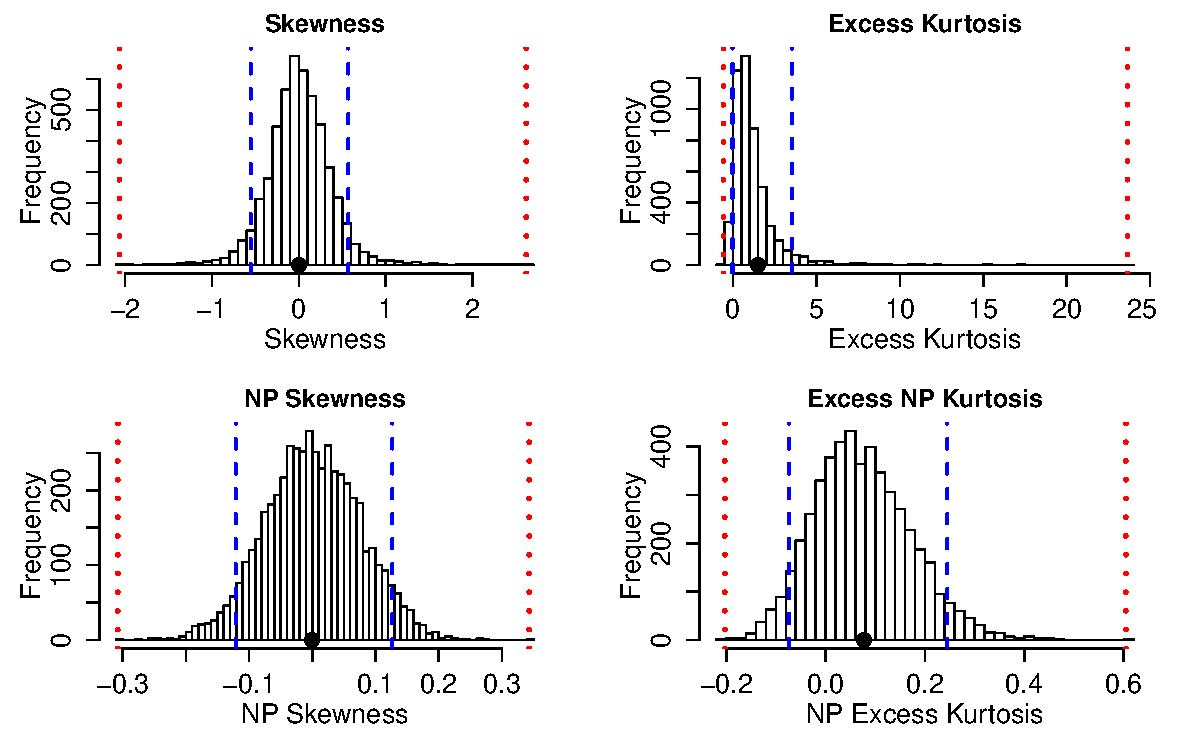
\includegraphics[width=\textwidth]{figures/NPmoments.pdf}
\caption{Histograms of skewness and kurtosis estimates using the usual moment-based definitions, compared with the nonparametric
skewness and kurtosis measures. Histograms are based on 5000 replicate draws of a sample of 200 independent values fron 
a $t$ distribution with 8 degrees of freedom. Dotted red vertical lines mark the range of sample estimates, 
and dashed blue lines show the 5th and 95th percentiles. The true value is indicated by a black dot on the $x$-axis.
Figure drawn by script \texttt{NPmoments.R}}
\label{fig:NPmoments}
\end{figure} 

We therefore use ``nonparametric'' (NP) measures of skew and kurtosis that are based on quantiles and therefore are 
less sensitive to a few extreme data values. Let $q_\alpha$ denote the $\alpha$ quantile of a distribution or sample (e.g., $q_{0.05}$ 
is the 5th percentile. For any $0 < \alpha < 0.5$ a quantile-based measure of skewness is given by \citep{mcgillivray-1986}
\be
\mbox{NP Skewness} = \frac{q_\alpha + q_{1-\alpha} - 2 q_{0.5}}{q_{1-\alpha} - q_\alpha}.
\ee
NP Skewness is a measure of asymmetry between the tails of the distribution above and below its median. The size of the upper
tail can be measured (for any given $\alpha$) by $\tau_U = q_{1-\alpha} - q_{0.5}$; for $\alpha=0.05$ this is the difference
between the 95th percentile and the median. The lower tail size is $\tau_L = q_{0.5} - q_\alpha$. The definition above
is equivalent to  
\be
\mbox{NP Skewness} = \frac{\tau_U - \tau_L}{(\tau_U + \tau_L)/2}.
\label{eqn:NPskew}
\ee
So an NP Skewness of $\pm 0.2$ says that the difference in tail sizes is 20\% of their average. The range of possible values 
is -1 to 1. Both $\alpha=0.25$ (sometimes called ``Kelly's skewness'') and $\alpha=0.1$ (``Bowley's skewness'') 
are common choices. We used $\alpha=0.1$, unless otherwise stated.  
 
An analogous quantile-based measure of kurtosis \citep{jones-etal-1994} is 
\be
\mbox{NP Kurtosis}  = \frac{q_{1-\alpha} - q_{\alpha}}{q_{0.75} - q_{0.25}}.
\label{eqn:NPkurt}
\ee
For $\alpha=0.05$, NP Kurtosis is the difference between the 95th and 5th percentiles, relative to the interquartile range. 
The numerator in \eqref{eqn:NPkurt} is the sum of $\tau_L$ and $\tau_U$ for the chosen value of $\alpha$. 
To facilitate interpretation, we scale NP Kurtosis relative to its value for Gaussian distribution, and substract 1. 
We call this ``NP Excess Kurtosis''. The value for a Gaussian distribution is zero. A value of 0.2 means that the tails
are (on average) 20\% broader than those of a Gaussian with the same interquartile range, and a value of -0.2 means that the tails
are (on average) 20\% narrower than a Gaussian with the same interquartile range. We calculate NP Kurtosis using $\alpha=0.05$ 
unless otherwise stated, to focus on the tail edges, but again this is somewhat arbitrary. 

Figure \ref{fig:NPmoments}C,D illustrate how, applied to exactly the same simulated samples, the NP measures of skewness and
kurtosis produce a smaller fraction of highly inaccurate estimates casued by a few extreme values in the sample. But also note
that, in contrast to the moment-based measures, numerically small values of the NP measures (e.g., 0.1 or 0.2) should not be
disregarded, because they are both scaled so that a value of 1 indicates extremely large departures from a Gaussian distribution. 

\section{Case study: Sea fan corals, \emph{Gorgonia ventalina}}
We begin with a simple example where current size is the only predictor of future size. \cite{bruno-etal-2011} developed
an IPM to understand the rise and fall of the \emph{Aspergillus sydowii} outbreak in Caribbean sea fan corals 
\emph{G. ventalina}. The model was based on repeated observations of marked corals in permanent transects at several sites 
near Akumal, Mexico, recording disease status (infected/uninfected) and the area of uninfected tissue. 
The epidemic peak had passed and disease incidence was already low, so infected fans were relatively infrequent. 
We therefore limit the analysis here to uninfected individuals. \citet{bruno-et-al-2011} found statistically significant year
and site effects, but as those explained a very small fraction of the variation in growth increments, they fitted a single growth
model to data pooled across years and sites. We do the same here. The pooled data set consists of 358 observed
size transitions. Script \text{AkumalCorals.R} contains the analysis. 

\begin{figure}[tbp]
\centering
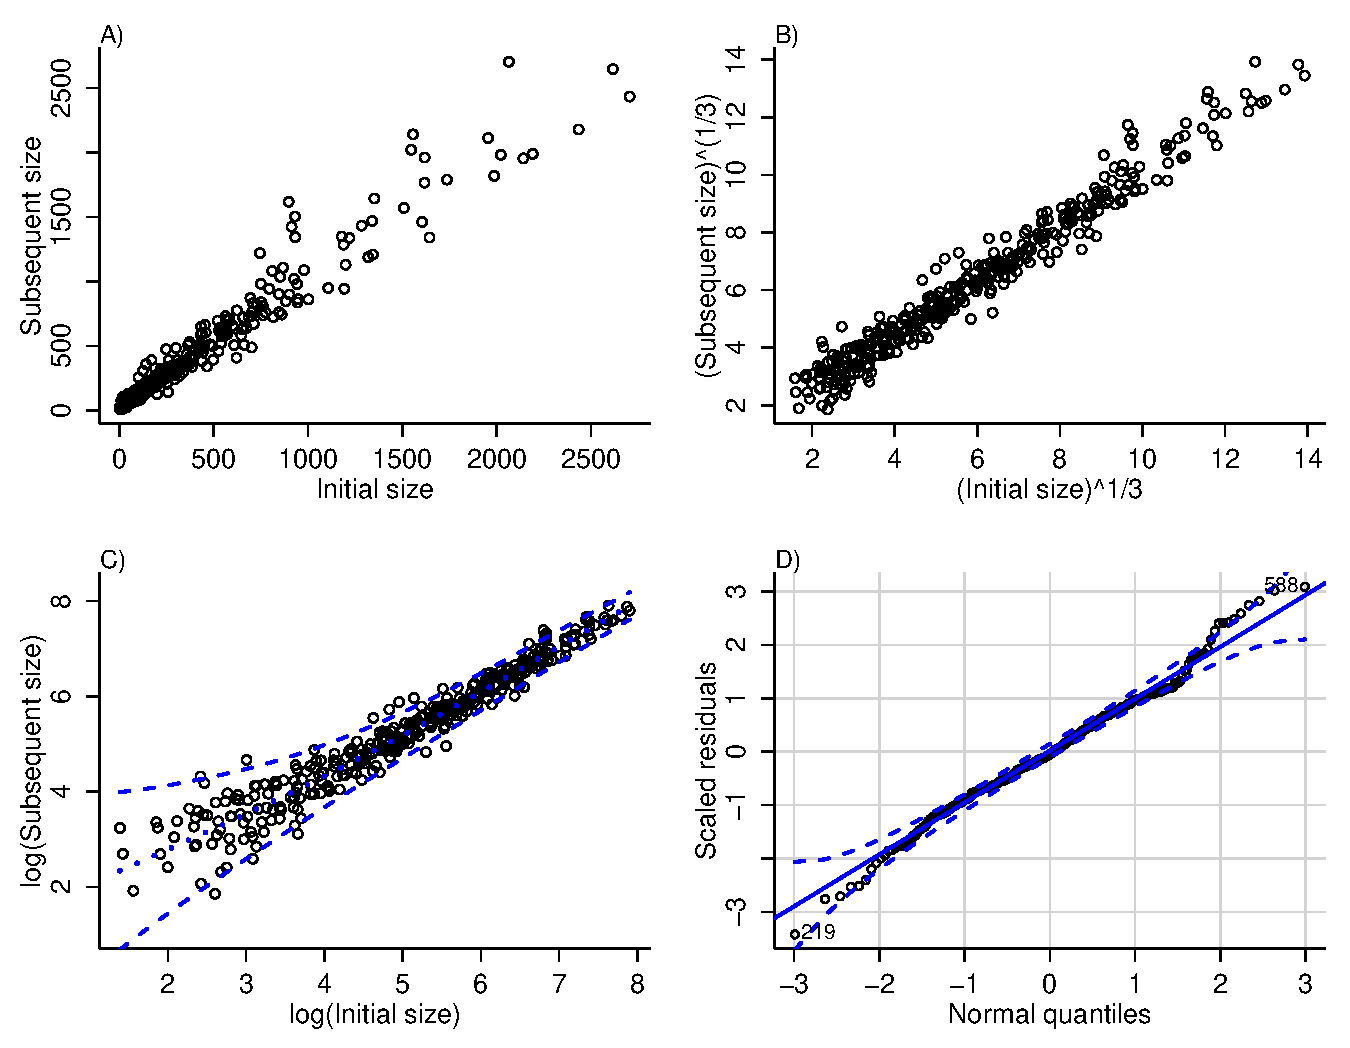
\includegraphics[width=\textwidth]{figures/AkumalPilot.pdf}
\caption{Pilot Gaussian model for growth of sea fan corals, \emph{Gorgonia ventalina}. \textbf{A)} Untransformed
data on size transitions. \textbf{B)} Size transitions on the cube-root scale used by \citet{bruno-etal-2011}. 
\textbf{C)} Size transitions on log scale, showing the mean (solid red curve) and mean$\pm 2$ standard deviations (blue dashed
curves) for the pilot Gaussian model with non-constant variance. \textbf{D)} Normal quantile-quantile plot of scaled residuals
from the pilot Gaussian model. Figure made by script \texttt{AkumalCorals.R}.}
\label{fig:AkumalPilot}
\end{figure} 

The data clearly exhibit size-dependent growth variance (fig. \ref{fig:AkumalPilot}A). 
\citet{bruno-etal-2011} chose to stabilize the variance by transforming size,
using the cube-root of total fan area as the size measure (fig. \ref{fig:AkumalPilot}B), and then fitting the standard 
model with Gaussian growth increments. But transformation only solves the one problem of size-dependent variance: residuals from 
the default model are non-Gaussian, and still exhibit significant skew and kurtosis ($p<0.01$ in Jarque-Bera Normality test, D'Agostino skewness test, 
and Anscombe-Glynn kurtosis test using R functions \texttt{jarque.test,agostino.test,anscombe.test} in the 
in the \textbf{moments} package \citep{komsta-2015}). This remains true in a model with site and year effects and 
site:year interaction. 

We therefore develop a model using log-transformation, which has two advantages. First, eviction at the lower size limit is
easily prevented by choosing a large negative value for minimum log area. Second, the distribution of recruit sizes is closer to Gaussian
on log scale than on cube-root scale (because the sample size is small both log- and cube root-transformed sizes are not significantly
non-Gaussian, but log-transformed data have smaller Jarque-Bera and Kolmogorov-Smirnov test statistics for non-normality). 

With initial size as the only predictor, the simplest way to fit a Gaussian model with nonconstant variance is the
\texttt{gam} function in \textbf{mgcv} library \citep{wood-2017} using the \texttt{gaulss} family. The mean and 
standard deviation are both fitted as smoothing spline functions of initial size, and the \texttt{predict} function
returns the fitted mean and also the inverse of the fitted standard deviations with which we can compute the scaled residuals: 
\begin{lstlisting}
# XH is a data frame holding the data
# logarea.t0, .t1 denote initial and final values of log-transformed area   
fitGAU <- gam(list(logarea.t1~s(logarea.t0),~s(logarea.t0)),
              data=XH,family=gaulss())
fitted_all = predict(fitGAU,type="response"); 
fitted_sd = 1/fitted_all[,2]; 
scaledResids = residuals(fitGAU,type=''response'')/fitted_sd;  
\end{lstlisting}
Fig. \ref{fig:AkumalPilot}C) shows the log-transformed data and Gaussian model. There are no visual signs of trouble,
but the scaled residuals are non-Gaussian (fig. \ref{fig:AkumalPilot}D; $p<0.03$ Jarque-Bera test for Normality).
There is little skew (skewness=0.06, $p=0.64$ D'Agostino test), but significant kurtosis (excess kurtosis 0.67, $p=0.03$ Anscome-Glynn test). 

We now need to find a better fitting distribution. The overall properties of the scaled residuals (as in the preceding
paragraph) may be misleading if the growth distribution changes as a function of initial size. 
For example, is skew is positive at small initial sizes and negative at large sizes, the overall distribution 
could have zero skew but positive excess kurtosis. A distribution family with those properties (e.g., a $t$ distribution) 
would be a bad fit to the conditional distribution of growth at any initial size. Thus, a pilot Gaussian model should not
be accepted just because the set of all scaled residuals is approximately Gaussian. 

\begin{figure}[tbp]
\centering
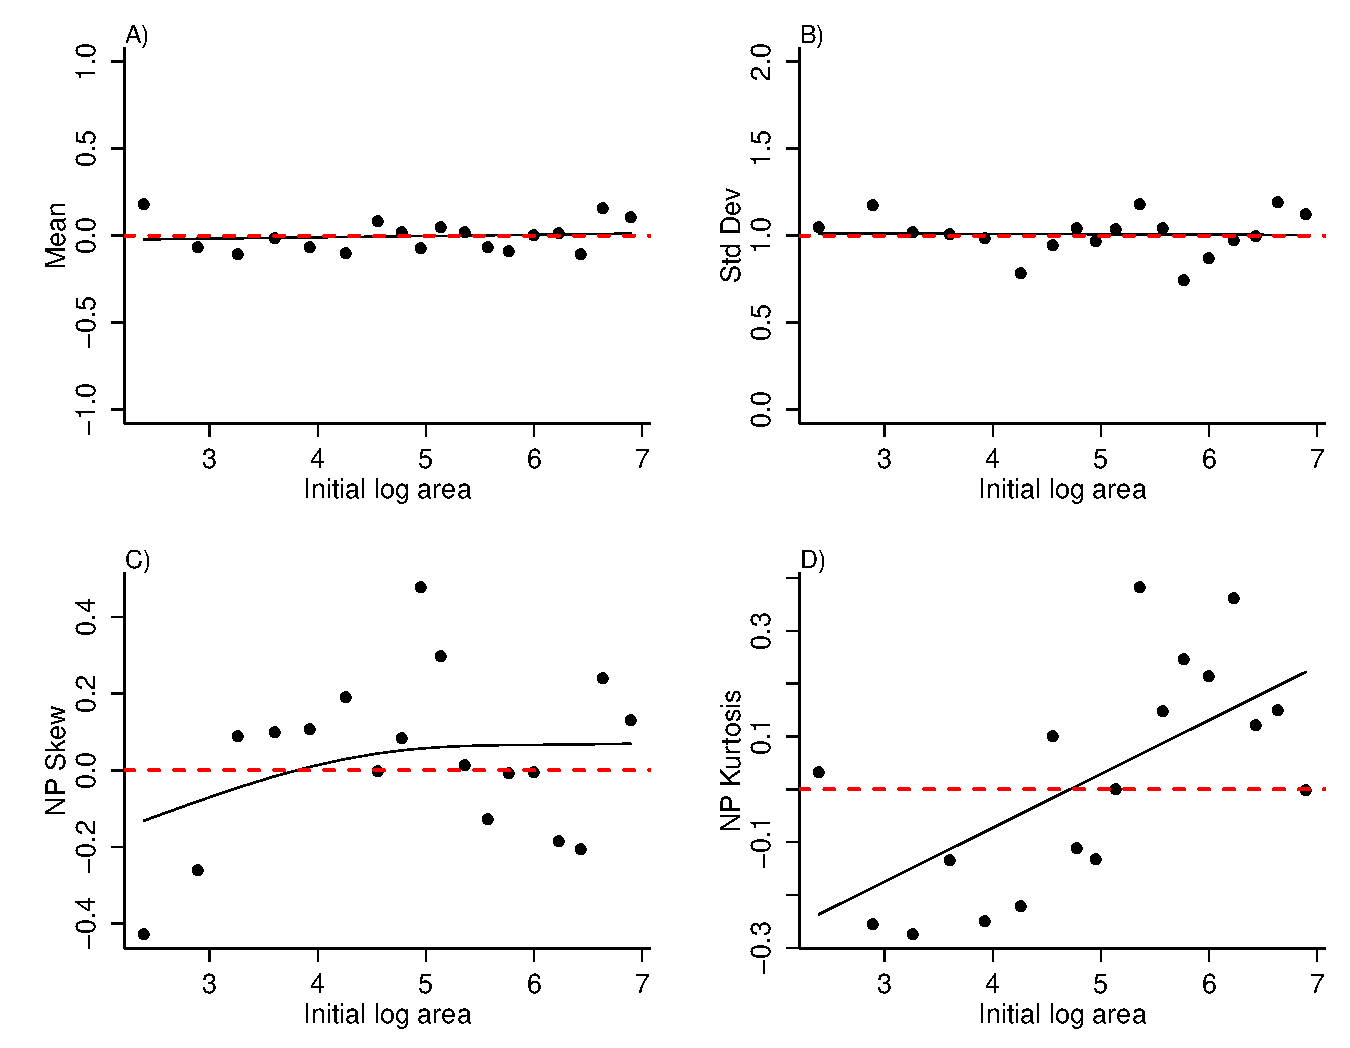
\includegraphics[width=0.8\textwidth]{figures/AkumalRollingResiduals.pdf}
\caption{Rolling moments plot for scaled residuals from the pilot Gaussian model for growth of sea fan corals, \emph{Gorgonia ventalina}. 
Figure made by scripts \texttt{AkumalCorals.R} and \texttt{Diagnostics.R}.}
\label{fig:AkumalRollingResiduals}
\end{figure} 

Instead, distribution choice should be guided by properties of distributions conditional on initial size. 
Rarely will data include many instances of multiple observations with identical initial sizes, but we can 
approximate conditional distribution by grouping similar initial sizes. 
In fig. \ref{fig:AkumalRollingResiduals}, summary statistics (mean, standard deviation, NP skewness, NP excess kurtosis) 
are plotted (solid points) for a set of sliding windows, each containing 10\% of the scaled residuals sorted according to initial size. 
The red dashed lines are what we would see if the pilot model were exactly right: zero mean, skewness and excess kurtosis, and standard deviation of one. 
Black curves are spline regressions through the points using \texttt{gam}. Panels A) and B) are a ``sanity check'' to verify
that the pilot model was adequate to capture the mean and variance of growth. Panel C) indicates that the overall low skew results from negative
skew at small sizes and positive skew at larger sizes. Similarly, panel D), reveals that NP kurtosis varies with initial size, 
negative for small fans (thin tails), positive at large sizes (fat tails). 

Fitting those properties requires a four-parameter distribution that allows nonzero skew, allows both 
positive and negative excess kurtosis, and whose range of possible values is $(-\infty, \infty)$. That narrows the options considerably. 
Of the more than 50 distributions available in the \textbf{gamlss.dist} package, the options are 
\texttt{EGB2, JSU, GT, SHASH} and four \texttt{SEP} distributions (four different ways of adding skew to the
exponential power distribution). We omit \texttt{SEP2} because it is known to have poorly identified parameters
\citep{diciccio-monti-2004}, which is problematic for diagnostics that we use in model selection. 

To choose among the candidate distributions, we sorted the scaled residuals based on initial size into 5 equal-size bins, 
and fitted all candidate distributions to each of the five resulting data sets by 
maximum likelihood\footnote{Our function \texttt{gamlssMaxlik} in online script \texttt{fitChosenDists.R} is
patterns after the \texttt{gamlss} function \texttt{gamlssML}, but uses the \texttt{maxLik} function from the \textbf{maxLik}
package \citep{maxLik-package}, and repeated optimization from different starting values, to increase the reliability of the results.} 
As all distributions have the same number of parameters, comparison of maximized likelihoods is equivalent to comparing AIC values. 
With the exception of \texttt{EGB2} all distributions had very similar maximized likelihoods for all bins; the best overall (summed
likelihood) was \texttt{SEP1}, so we proceeded with \texttt{SEP1}. 

Most four-parameter distributions have the inconvenient property that their parameters are \emph{not} the mean, standard deviation, skew,
and kurtosis of the distribution. This happens because (for example) introducing nonzero skew changes the mean and the kurtosis. 
So to see how distribution parameters vary as a function of initial size, instead of inspecting fig. \ref{fig:AkumalRollingResiduals}, we need
to look directly at how parameters vary as a function of initial size. As before, we did this by binning the data based on initial sizee, 
and fitting an \texttt{SEP1} distribution to the subsequent size values in each data subset. Note, 
in fig. \ref{fig:AkumalRollingResiduals} we used scaled residuals as the response variable, 
to minimize how variation in mean and standard deviation within a bin would affect the skew and kurtosis. 
Here, because all four distribution parameters interact to determine the distribution, we need to fit all 
four simultaneously to the data on subsequent size in each bin. 

As expected from the pilot Gaussian fit, the location parameter $\mu$ and the log of the scale parameters $\sigma$ appear to
vary linearly with initial size. The skewness parameter $\nu$ and log of the kurtosis parameter $\tau$ also appear to
vary linearly (note: log is the default link function for $\sigma$ and $\tau$ in \texttt{SEP1} because both must be positive).  

\begin{figure}[tbp]
\centering
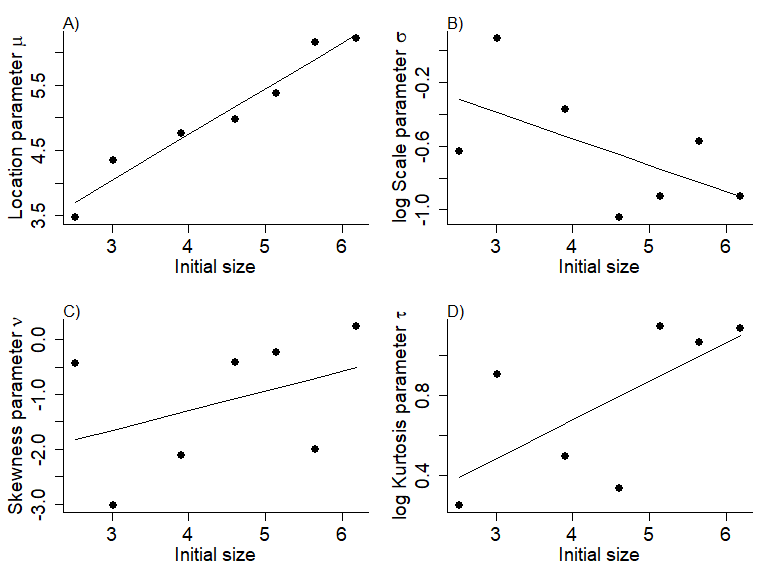
\includegraphics[width=0.8\textwidth]{figures/RollingSEP1parsCorals.png}
\caption{Binned data SEP1 parameter estimates for growth distributions of sea fan corals, \emph{Gorgonia ventalina}. 
Figure made by scripts \texttt{AkumalCorals.R} and \texttt{Diagnostics.R}.}
\label{fig:AkumalRollingSEP1pars}
\end{figure} 

Our candidate model for the overall growth kernel is thus an \texttt{SEP1} distribution in which $\mu, \log \sigma, \nu$ and $\log \tau$
are all linear functions of initial size. This is easily fitted by maximum likelihood, using the pilot Gaussian fit and 
the values plotted in fig. \ref{fig:AkumalRollingSEP1pars} to inform the starting parameter values. 

The ``acid test'' of a growth model is that simulations from the fitted model should look like the real data. 
To implement that criterion, we compared simulated and actual data with respect to quantiles of the distribution
of subsequent size, again using a series of bins defined by initial size to account for how those quantiles vary
with initial size. The candidate model described was not an unequivocal success -- there were
discrepancies in the smaller bins, for several of the quantiles, mostly in the same direction. This suggests that
the predicted mean is the source of the problem, so we modified the candidate model by adding a quadratic term
for the location parameter. This resulted in a near-exact correspondence between model simulations and the
data at all quantiles for all bins; moreover, the added quadratic terms was highly significant in the maximum
likelihood fit ($p<0.001$). 


 

\clearpage   

\section{Case study: bunchgrass, \emph{Pseudoroegneria spicata}}

We again consider a species where one of us is the offender -- initially using the default model because 
it was hard to do better at the time \citep{adler-etal-2010}, but sticking with it 
\citep[e.g.,][]{Tredennick2018, Adler-2018} when it would have been easy to do better.   

NOTE: for now, this is just an outline of methods and results. 

We used the most recently curated version of the data \citep[][at doi.org/10.5061/dryad.96dn293]{Adler-2018},
both legacy (22 annual transitions between 1926 and 1957) and modern (8 annual transitions from
2008 to 2016, excluding moisture manipulation treatments). We excluded seedlings, which require separate models
\citep{Chu-2014a, Chu-2015, snyder-ellner-2018}, and individuals mapped as ``too small to measure'' that should be modeled separately
as a discrete size category (though in the past we have not done that). The measure of plant size was log basal cover. 
Based on past analyses, (1) we did not distinguish between historical and 
modern Control treatments \citep{Adler-2018} (2) we included size by year interactions with year-specific slope and intercept
for a linear relationship between current and future size (log basal cover); (3) Quadrat group (labeling sets of spatially
nearby quadrats), Treatment (Control or Shrub removal) and competition with other species were included as covariates. 
As in past models, competition was measured by distance-weighted cover of competing species, using nonparametric competition
kernels estimated from the data \citep{Teller-2016}. 

The ``pilot'' model (Gaussian) was constructed using \texttt{lmer} with annual slope and intercept specified 
as random effects, using iterative re-weighting to fit a model with non-constant variance (exponential function of fitted value). 
It also included a quadratic term in initial size, based on residual diagnostics of a model without the quadratic term. 

Results: \begin{enumerate}

\item Model selection for the ``pilot'' model was limited to the competition effects,  
using AIC values as reported by \texttt{lmer}). The selected model had  
three competition covariates: (1) the shrub \emph{Artemisia tripartita}, (2) the other two dominant 
bunchgrasses combined, and (3) all other species combined. 

\item The set of all scaled residuals was non-Gaussian, based on quantile-quantile plot, mostly in the lower tail. Statistical tests
confirmed that the distribution was non-Gaussian, skewed and fat-tailed (all $P<0.001$). 

\item Rolling moments diagnostics applied to the scaled residuals (Fig. \ref{fig:rollingMomentsPSSP}) show that the mean 
and Std Dev are nearly constant as a function of the fitted value (conditional mean), as they should be. The small trend in 
the mean shows that the regression coefficients are slightly biased, which is not unexpected because the Gaussian assumption is violated. 
In contrast, there are large trends in the skew and kurtosis. 

\begin{figure}[tbp]
\centering
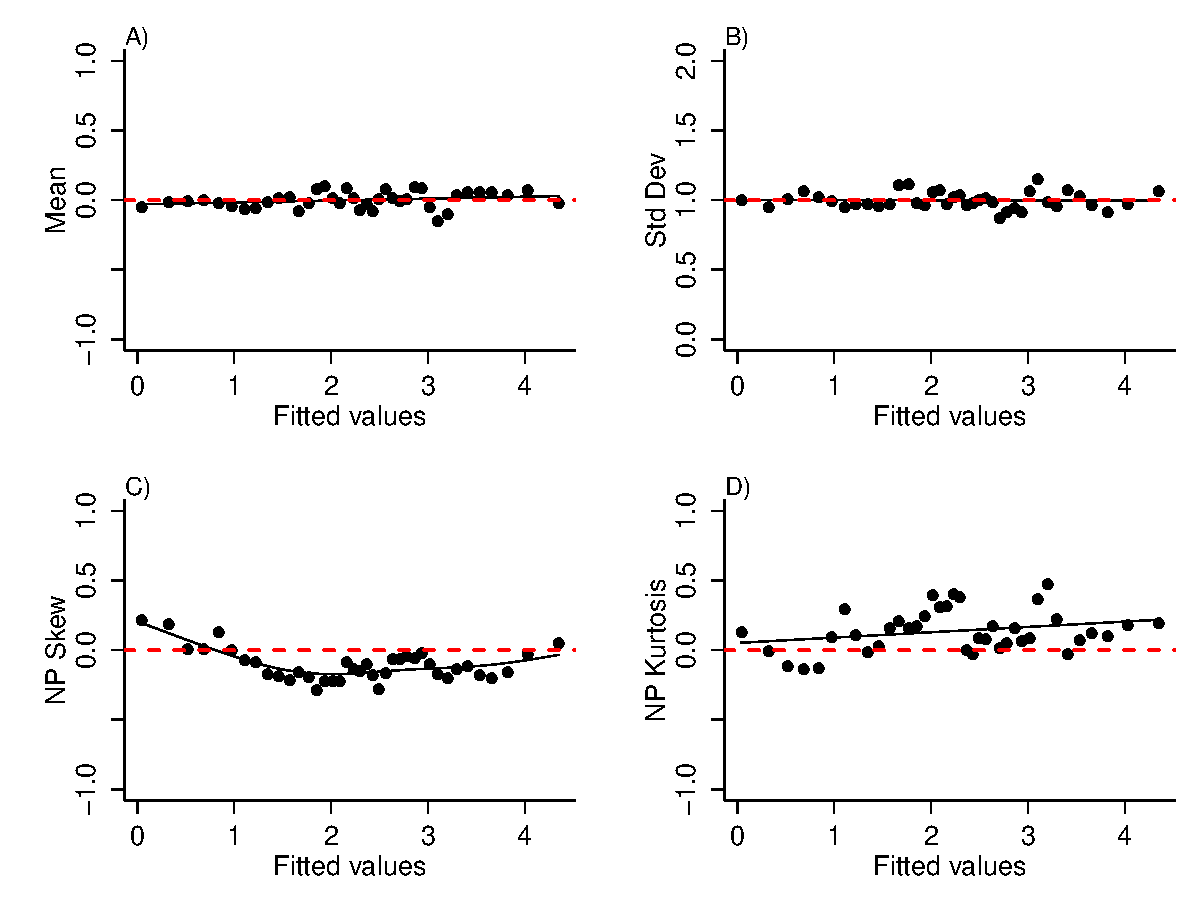
\includegraphics[width=.9\textwidth]{figures/RollingNPMomentsPSSP.pdf}
\caption{Rolling moments of scaled residuals from the pilot model, as a function of fitted
values, for \emph{P. spicata}. The dashed red line is the value expected if the pilot model fits the
data, in particular skew=0 and kurtosis=3.}
\label{fig:rollingMomentsPSSP}
\end{figure} 

\item Because the skew and kurtosis are variable, it is not informative to find a distribution that fits
the entire set of scaled residuals. For example: a mixture of distributions, some with positive skew and some
with negative, is likely to have very high kurtosis even if none of the component distributions does. So selecting
a distribution family can't just be turned over to \texttt{fitDist}. 

Instead, we have to ask: what families are flexible enough to accomodate the features in Fig. \ref{fig:rollingMomentsPSSP}?
We need at least 4 parameters (mean, variance, skew, kurtosis) -- JSU, SHASH the various skew $t$ distributions 
are convenient options. Moreover,the family must allow both positive and exactly zero excess kurtosis relative to a Gaussian. 
In JSU and skew $t$ that makes fitting problematic, because exactly zero excess kurtosis only occurs as a limit, not at 
any actually possible parameter values ($df \to \infty$ for $t$, and $\tau \to 0$ for JSU). So let's try SHASH, which covers most
of the mathematically possible set of (skew, kurtosis) combinations (see Jones \& Pusey 2009).  

\item SHASH has the problem that the location parameter $\mu$ is not the ``fitted value'' (distribution mean), $\sigma$ is not actually
the standard deviation, $\nu$ is not actually the skew, and $\tau$ is not actually the kurtosis. We can't figure out how to model 
the variation in those parameters by looking at variation in moments of the pilot residuals, or of anything else for that matter. 

So instead, I broke the data into even-size bins based on fitted values of the pilot model, and fitted a SHASH distribution to
the set of final sizes, Fig. \ref{fig:rollingSHASHparsPSSP}. Panel A), $\mu$ as a function of the fitted values, doesn't really inform
modeling, but it shows that $\mu$ can be regarded as a ``fitted value''. The other plots tell us how the other distribution parameters
should be modeled as a function of $\mu$, which is what we need to write down the growth model likelihood: $\sigma$ and $\tau$ are linear,
$\nu$ is quadratic. 
 
\begin{figure}[tbp]
\centering
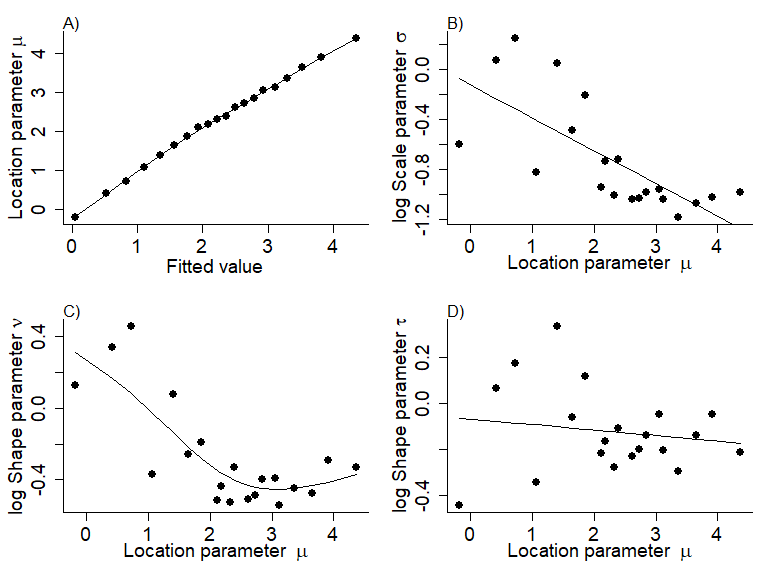
\includegraphics[width=.9\textwidth]{figures/RollingSHASHparsPSSP.png}
\caption{Binned data SHASH parameters plot for \emph{P. spicata}. }
\label{fig:rollingSHASHparsPSSP}
\end{figure} 

\item The model is easy to fit by ML. Used \texttt{maxLik}, which allows the \texttt{BHHH} optimization method that seems to be faster 
than anything \texttt{mle} or \texttt{bbmle} can use. Now, does it do a good job of fitting the data? 

\begin{figure}[tbp]
\centering
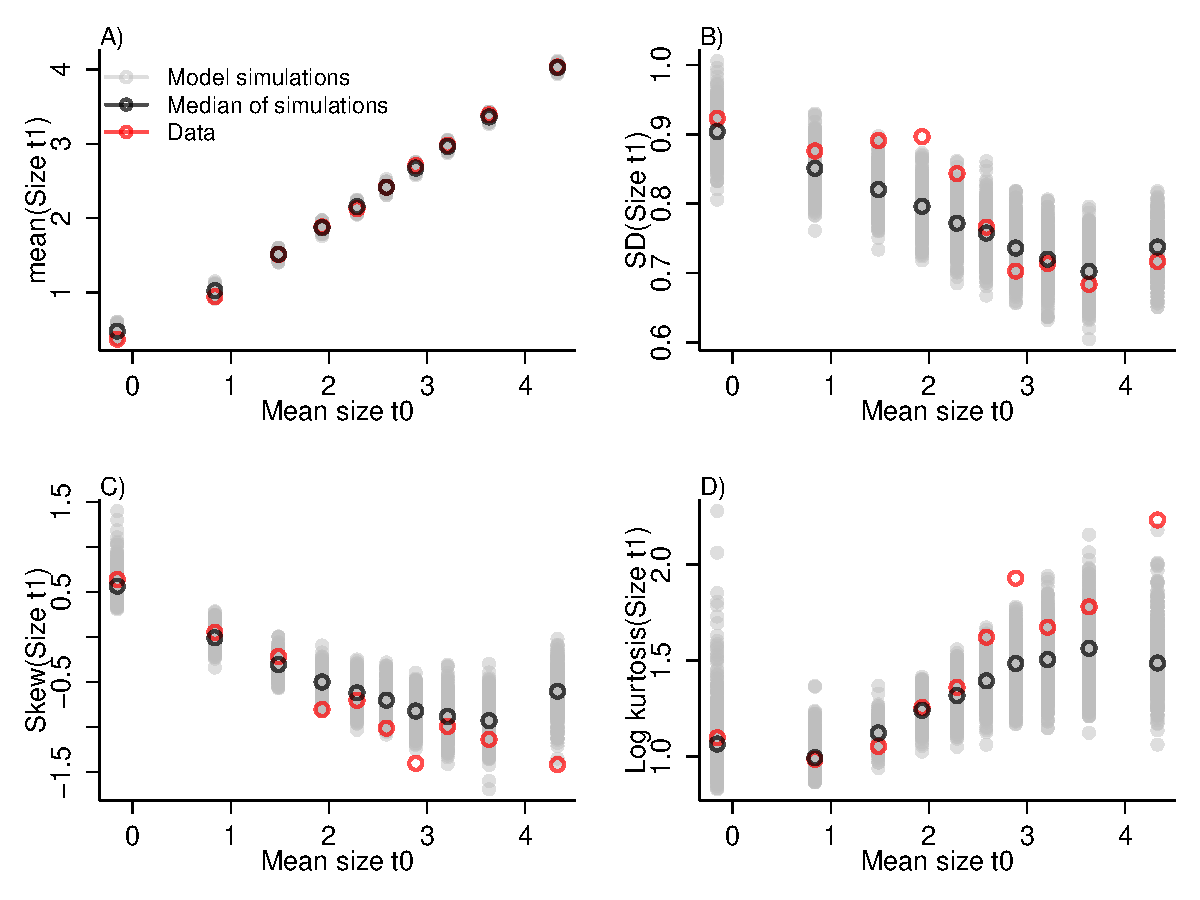
\includegraphics[width=.9\textwidth]{figures/BinnedConditionalMoments.pdf}
\caption{Binned data comparison of moments between simulations of the fitted SHASH model (grey, black) and the actual data (red) for 
{P. spicata}. Individuals were binned based on their initial size. }
\label{fig:BinnedConditionalMoments}
\end{figure} 

\begin{figure}[tbp]
\centering
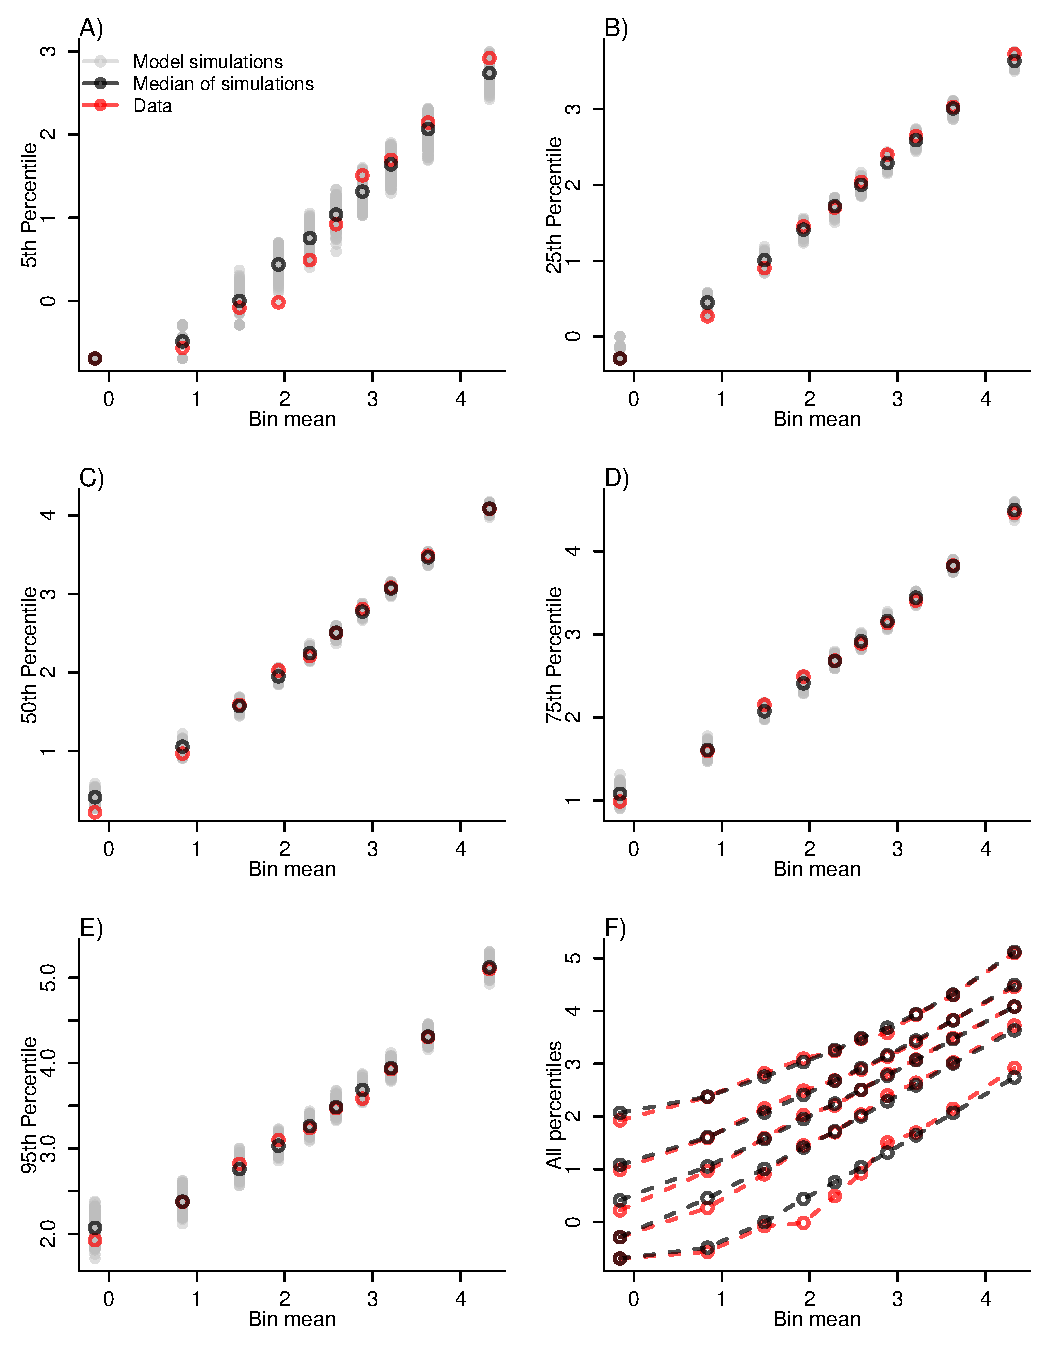
\includegraphics[width=.9\textwidth]{figures/BinnedConditionalQuantiles.pdf}
\caption{Binned data comparison of distribution quantiles between simulations of the fitted SHASH model (grey, black) and the actual data (red) for 
{P. spicata}. Individuals were binned based on their initial size. }
\label{fig:BinnedConditionalQuantiles}
\end{figure} 

Figures \ref{fig:BinnedConditionalMoments}  and \ref{fig:BinnedConditionalQuantiles} show two comparisons between the actual data and simulations
of the fitted SHASH model (i.e., repeated draws of subsequent size for all individuals in the data set), for a series of bins defined by initial
size. The comparison based on quantiles (fig. \ref{fig:BinnedConditionalQuantiles}) looks really good. The one based on moments is less good. 

The real-data moments exhibit some ``random'' variability -- e.g., not a steady trend in skew and kurtosis -- so perhaps they are being
dominated by a few outliers? Maybe that plot is unduly pessimistic, and to really ask if the model is consistent with the data we should 
ad bootstrap samples from the data as multiple pink dots analogous to the multiple grey dots for the model simulations. 

\begin{figure}[tbp]
\centering
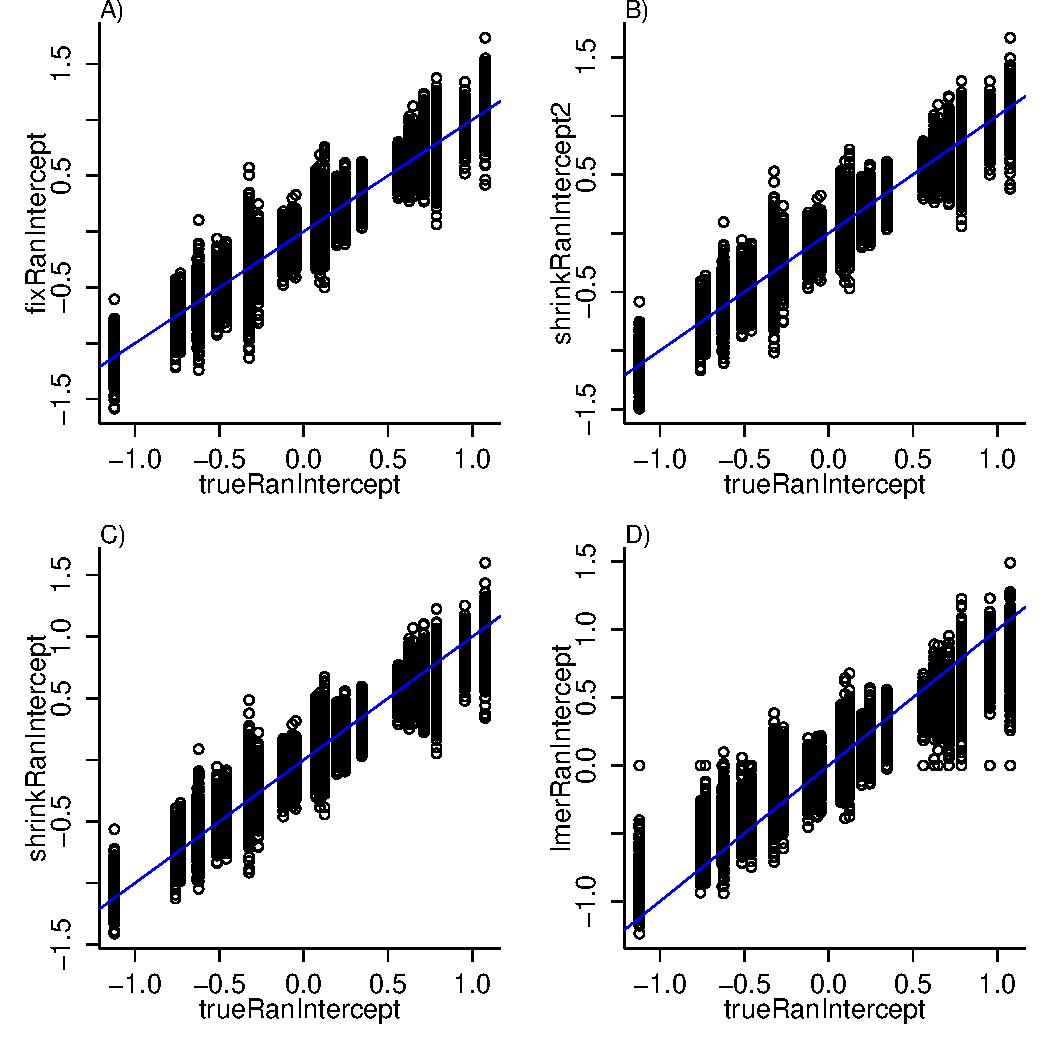
\includegraphics[width=.9\textwidth]{figures/ShrinkageTest.pdf}
\caption{Comparison of ``true'' and estimated intercept year effects for {P. spicata}. }
\label{fig:ShrinkageTest}
\end{figure} 


\item Finally, a simulation study was done to see how well the shrinkage approach recovers known year effects. Fig. \ref{fig:ShrinkageTest}
illustrates the results for the intercept coefficient. Panels A,B,C,D are the fixed-effects estimates, recommended shrunk estimates,
more strongly shrunk estimate, and estimates from \texttt{lmer}. Except for \texttt{lmer} they all look pretty similar, and they are,
but the recommended shrunk estimates had the lowest mean-square error for both slope and intercept (averaged across all years),
and their sample variance was closest to the across-year variance in the data-generating model. So shrinkage is barely worth doing, but
it's easy and it does make a small improvement. 

\end{enumerate} 




\section*{Acknowledgements} 
This research was supported by US NSF grants DEB-1933497 (SPE) and .... 

%\bibliographystyle{EcologyLetters}
\bibliographystyle{apalike}
\bibliography{BetterGrowthModeling}

% ######################## Appendices ##############################
\newpage 
\clearpage 
% \setcounter{page}{1}
\setcounter{equation}{0}
\setcounter{figure}{0}
\setcounter{section}{0}
\setcounter{table}{0}
\setcounter{Box}{0}
\renewcommand{\theequation}{S.\arabic{equation}}
\renewcommand{\thetable}{S-\arabic{table}}
\renewcommand{\thefigure}{S-\arabic{figure}}
\renewcommand{\theBox}{S-\arabic{Box}}
\renewcommand{\thesection}{S.\arabic{section}}

\centerline{\Large{\textbf{Appendices}}}

\section{Estimating mixed-effects models using shrinkage}

Ecologists often fit demographic and other statistical models that include random effects terms to
quantify variation among years, spatial locations, individuals, etc. Random effects
are a natural choice when interest centers on the magnitude of variation (e.g., how much does mortality vary among years?)  
rather than individual values (e.g., mortality in 2013). They also allow each estimate to 
``borrows strength'' from others, so that (for example) the estimate from a year with small sample size (and thus large 
sampling variability) is shifted towards the center of the overall distribution. 

Specialized software is often used to fit such models, such as the \textbf{nlme, lme4, mgcv} and \textbf{gamm4} libraries in R,  
but these only allow a small subset of the distribution families we want to consider for modeling growth increments (the \textbf{gamlss} 
package allows many distribution families, but in our experience, even when random effects are simple in structure 
the fitting algorithms often fail to converge or fail to find the global optimum). 

One way past this limitation is Bayesian estimation, using STAN with user-written (or borrowed) 
code for the chosen growth distribution (see section XX for an example). 
In this appendix we describe another option, introduced by \citet{link-nichols-1994} and \citet{gould-nichols-1998}: 
fitting a fixed-effects model by Maximum Likleihood, followed by shrinkage of coefficient estimates. 
None of the ideas here are original. The material overlaps Appendix S1 of \citet{metcalf-etal-2015}, 
but for completeness we make it self-contained. Appendix D of \citet{cooch-white-2020} (written by K.D. Burnham)
provides more details and examples in the context of capture-recapture analysis. 

Here we explain shrinkage using a simple model based on our analysis of \emph{Pseudoroegneria spicata}. 
That model includes random effects for between-year variation in the slope and intercept of future size 
(log area) as a function of initial size. To keep the example simple, we assume that initial size 
and year are the only covariates, and we assume that growth increments 
follow a skew-Normal distribution with nonconstant variance and constant skew parameter. 
Code for this example is in the script \texttt{SimpleShrinkageExample.R}. The first part of the script generates
an artificial data set by fitting the model to a subset of the growth data (20th century Control plots), and
randomly generating new ``size next year'' values for each individual in the actual data set. 
The second part contains the ``data'' analysis. 

As in our \emph{P. spicata} analysis, we assumed that that the skew and kurtosis parameters were functions
of the location parameter; this dominated $(\Delta AIC \approx 30)$ the alternate 
model with skew and kurtosis depending on initial size.   
The analogous Gaussian model, with constant variance, could be fitted as follows using \texttt{lmer}:
\begin{lstlisting}
lmer(new.size ~ init.size + (init.size|year), data=growthData, REML=TRUE); 
\end{lstlisting}
where \texttt{growthData} is a data frame holding the data with \texttt{year} as an unordered factor. For our skew-Normal
model, we instead use maximum likelihood with all between-year variation included as fixed effects. The appropriate design
matrix is easily constructed using the \texttt{model.matrix} function: 
\begin{lstlisting}
U = model.matrix(~year + init.size:year - 1, data=growthData)
\end{lstlisting}
If there are $T$ years, the matrix \texttt{U} specified in this way has $2T$ columns corresponding to $n$ annual 
intercepts and $T$ annual slopes. 

Using this design matrix, we can readily write a log likelihood function for use with 
the \textbf{maxLik} package, with a log link function for the variance because it is necessarily positive: 
\begin{lstlisting}
LogLik=function(pars,new.size,U){
    pars1 = pars[1:ncol(U)]; pars2=pars[-(1:ncol(U))];
    mu = U%*%pars1;  
    sigma = exp(pars2[1]+pars2[2]*mu);
    dSN1(new.size, mu=mu, sigma=sigma, nu=pars2[3], log=TRUE)
}
\end{lstlisting} 

Parameters and their standard errors can then be estimated with \texttt{maxLik}, 
starting from a random guess: 
\begin{lstlisting}
start=c(runif(ncol(U)), rep(0,3))
out=maxLik(logLik=LogLik,start=start, new.size=simData$new.size,U=U,
  method="BHHH",control=list(iterlim=5000,printLevel=1),finalHessian=TRUE);
coefs = out$estimate; # parameters
V = vcov(out); SEs = sqrt(diag(V));	# standard errors 
\end{lstlisting}  
In real life we would repeat the optimization several times with several different starting values, to be confident that
the optimal parameter values had been found. 

Focus now on the year-specific intercept parameters $\hat{a}_t, t = 1,2,\cdots T$. 
We can view the year-specific estimates $\hat{a}_t$ as consisting of unobserved true values $a_t$ plus sampling error:
\be
\hat{a}_t= a_t + \varepsilon_t 
\ee
Because of the sampling errors, the sample variance of
the estimates $\hat{a}_t$ is an upward-biased estimate of the true across-year variance in the parameter. 
That is undesirable if the model will be used to project how temporal variability affects population dynamics. 
However, maximum liklihood estimation gives us an approximaten variance-covariance matrix $\hat{V}$ of the
sampling errors, \texttt{V} in the code above. With that information, we can estimate the parameters
of a random effects model for the intercept parameters, and thereby improve the year-specific estimates and
the estimate of the across-year variance.  

The model is as follows. We make the standard mixed-models assumptions that the $a_t$ are drawn 
independently from some fixed distribution with unknown variance $\sigma^2$. We also assume that the estimates 
$\hat{a}_t$ are unbiased, that is
\be
\mathbb{E}(\varepsilon_t \vert a_t) = 0.    
\ee
These are optimistic assumptions, but not excessively optimistic. Some degree of temporal correlation will often be
present, and as we explain at the end, it is theoretically possible to account for it. 
Maximum likelihood parameter estimates are not unbiased, but if the assumptions
of maximum likelihood are satisfied the bias is asympototically negligible compared to the standard error (the 
bias scales as the inverse of sample size, the standard error as the square root of the inverse of sample size).  

Let $S^2$ denote the sample variance of the estimates $\hat{a}_t$. It can then be shown that 
\be
\mathbb{E}(S^2) = \sigma^2  + \frac{1}{T}\sum\limits_{t=1}^T \mathbb{E} Var(\varepsilon_t) 
- \frac{1}{T(T-1)}\sum\limits_{i=1}^{j-1} \sum\limits_{j=1}^T \mathbb{E}Cov(\varepsilon_i, \varepsilon_j). 
\label{eqn:biasTerms}
\ee
This is eqn. (1) in \citet{gould-nichols-1998} in our notation, without the term that 
results from temporal autocorrelation. 

The terms besides $\sigma^2$ on the right-hand are the expected impact of sampling error on the across-year variance
of the parameter estimates; their presence makes $S^2$ a biased estimated of $\sigma^2$. However,
all of those terms correspond to entries in the variance-covariance matrix $V$. We can therefore use our estimated
variance-covariance matrix $\hat{V}$ to removes the bias due to sampling variability: 
\be
\hat{\sigma^2}  = S^2 - \frac{1}{T}\sum\limits_{t=1}^T \hat{V}_{t,t} + 
\frac{1}{T(T-1)}\sum\limits_{i=1}^{j-1} \sum\limits_{j=1}^T \hat{V}_{i,j}. 
\label{eqn:hatSigma}
\ee
$\hat{\sigma^2}$ estimates the variance of the distribution from which the $a_t$ are assumed
to be drawn. 

Using that estimate, we can adjust the year-specific estimates to reduce the expected 
impact of sampling error. Depending on your purposes, there are two possible adjustments. 
The first option is the one used in the popular capture-recapture analysis 
software Mark \citet{cooch-white-2020}, 
\be
\widetilde{a}_t = \bar{\hat{a_t}} + \sqrt{\frac{\hat{\sigma}^2}{\hat{\sigma}^2 + \hat{V}_{t,t}}}\left (\hat{a_t} - \bar{\hat{a_t}} \right). 
\label{eqn:ShrinkLess}
\ee
The name ``shrinkage'' comes from the fact that each estimate is adjusted towards the overall mean, with 
larger adjustments of values that have higher estimated sampling error variance, $\hat{V}_{t,t}$. 
This shrinkage estimate has the property that the expected sample variance of the 
adjusted estimates $\widetilde{a}_t$ is very close to $\hat{\sigma^2}$, so the $\widetilde{a}_t$ approximate
the actual amount of 

The second is to replace $\hat{a}_t$ by the least-squares estimate of $a_t$ under the 
additional assumption that the $a_t$ are drawn from a Gaussian distribution; this is given by 
\be
\widetilde{a}_t = \bar{\hat{a_t}} + \frac{\hat{\sigma}^2}{\hat{\sigma}^2 + \hat{V}_{t,t}}\left (\hat{a_t} - \bar{\hat{a_t}} \right). 
\label{eqn:ShrinkMore}
\ee
This option is theoretically preferable if you are mainly interested in year-specific values rather than the across-year variance,
and the Gaussian assumption is reasonable. However, \citet{metcalf-etal-2015} found that even \eqref{eqn:ShrinkLess}, which does 
less shrinkage, resulted in a small downward bias in the temporal variance of population growth rates. This argues for  
always using the first option, as MARK does, and we do the same here. 

We differ from MARK, however, in using \eqref{eqn:hatSigma} rather than an iterative method that takes \eqref{eqn:hatSigma} as its 
starting estimate and refines the estimate by using weighted least squares based on the current estimate. 
\citet{metcalf-etal-2015} found, in simulation studies, that the iterative method was usually slightly beneficial but 
sometimes wildly inaccurate. We therefore advise against it. 

Finally, as mentioned above, the estimate of $\sigma^2$ can account for temporal autocorrelation in the $a_t$. 
When present, those correlations add a term to eqn. \eqref{eqn:biasTerms} (see eqn. (1) in \citet{gould-nichols-1998}), 
which can be estimated from the sample autocorrelation of the $\hat{a}_t$. We do not recommend doing this (and therefore omit
the formulas) because the autocorrelations can only be reliably estimated if they fall to nearly zero within lag $m \ll T$, in which
case the autocorrelation term is small (specifically, $O(m/T)$). Otherwise, the random error from using poorly estimated 
autocorrelations is likely to outweight the small bias from omitting that term. 

The take-home message is that estimating random effects from the regression coefficients is very simple: 
\begin{lstlisting}
# Variance-covariance matrices for intercepts and slopes
V1 = V[1:T,1:T]; V2 = V[(T+1):(2*T),(T+1):(2*T)]; 
# Extract year-specific intercepts, center them to zero   
fixed.fx = coefs[1:T]; fixed.fx = fixed.fx-mean(fixed.fx); 

# Estimate sigma^2
var.hat = mean(fixed.fx^2) - mean(diag(V1)) + 
              (sum(V1)-sum(diag(V1)))/(2*T*(T-1)); 

# Shrink deviations from the mean 
shrinkRanIntercept = fixed.fx*sqrt(var.hat/(var.hat + diag(V1)));

# Do it all again for the slopes 
fixed.fx2 = coefs[(T+1):(2*T)]; fixed.fx2 = fixed.fx2-mean(fixed.fx2); 
var2.hat = mean(fixed.fx2^2) - mean(diag(V2)) + 
               (sum(V2)-sum(diag(V2)))/(2*T*(T-1)); 
shrinkRanSlope = fixed.fx2*sqrt(var2.hat/(var2.hat + diag(V2))); 
\end{lstlisting}

The figure below shows the results for one artificial PSSP ``data'' set, having $T=22$ years and growth measurments on 
about 175 individuals/year on average. The true random year effects (the ones used to generate the data) are recovered
with good accuracy and no bias. In particular there is no sign of extreme values being pulled in too far
towards the mean, which would cause an S-shaped graph of estimated versus true values. 

\centerline{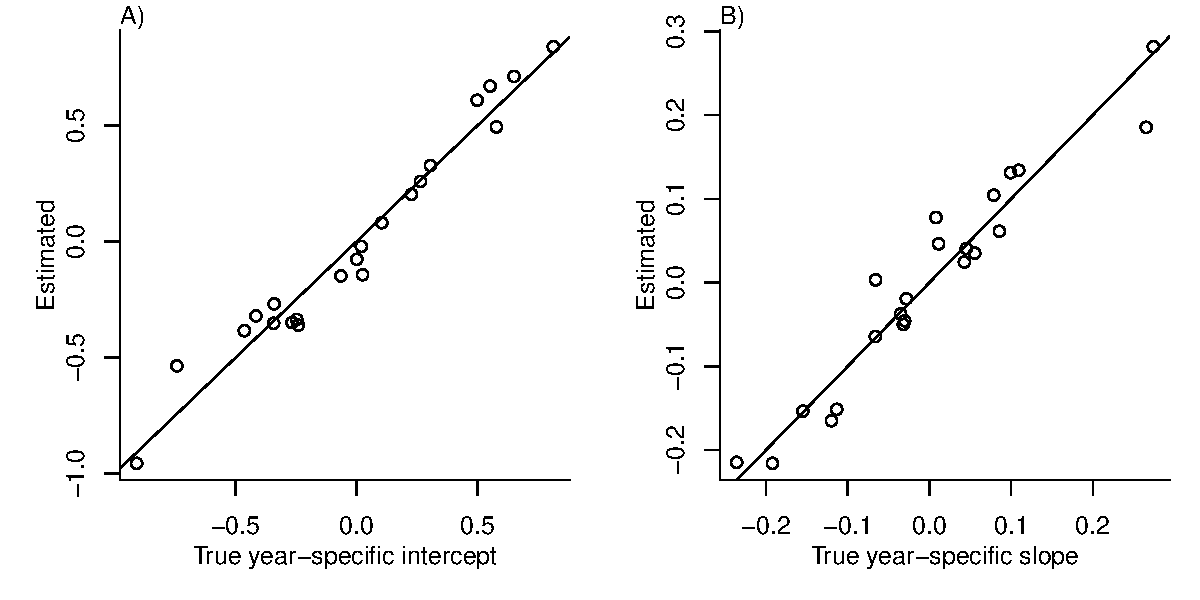
\includegraphics[width=\textwidth]{figures/SimpleShrinkage.pdf}}

  
\end{document}